\documentclass{beamer}

\title{Data Generating Processes and Statistical Modeling}
\author{Jeffrey B. Arnold}
\date{January 28, 2016}

\usepackage{tikz}

\begin{document}

\begin{frame}
  \maketitle{}
\end{frame}

\begin{frame}
  \frametitle{Data Generating Processes (DGP)}

  \begin{center}
  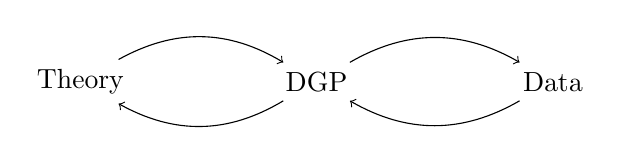
\begin{tikzpicture}[scale=1.5]
    \node (theory) at (-2, 0) {Theory} ;
    \node (dgp) at (0, 0) {DGP} ;
    \node (data) at (2, 0) {Data} ;
    \draw [->] (theory) to [bend left] (dgp);
    \draw [->] (dgp) to [bend left] (data);
    \draw [->] (data) to [bend left] (dgp);
    \draw [->] (dgp) to [bend left] (theory);
  \end{tikzpicture}
  \end{center}

  \begin{quote}
    [A] \textit{data generating process} (DGP) is rule or set of rules governing the social or political events that an analyst wishes to study and the rules by which observations of its results come to be represented in a dataset. A DGP \dots{} governs how a factors in a political process are related to each other. \textit{SMISS} (p. 70)
  \end{quote}

\end{frame}

\begin{frame}
  \frametitle{DGP: Stochastic vs. Deterministic}
  
  \begin{itemize}
  \item \textbf{Deterministic}: sufficient and necessary conditions to observe data
  \item \textbf{Stochastic}: probability of observing the data
  \item Why treat DGP as stochastic?
    \begin{itemize}
    \item Sampling uncertainty
    \item Theoretical uncertainty
    \item Fundamental uncertainty
    \end{itemize}
  \end{itemize}
\end{frame}

\begin{frame}
  \frametitle{DGP and Statistical Models}

  \begin{itemize}
  \item Stochastic DGP treats data as random variables
  \item Theoretically interested in specific parameters of the random variable: expectation
  \item \textit{Model-based sampling}: assume a specific parametric probability distribution
  \item Problems with \textit{model-based sampling}: DGP adds additional structure not implied by theory
  \end{itemize}
  
\end{frame}

\begin{frame}
  \frametitle{Statistical Model with a Normal Distribution }
  
  \begin{align*}
    Y &= \mu + \epsilon \\
    \epsilon & \sim N(0, \sigma) \\
    \mu &= \alpha + \beta X
  \end{align*}

  \begin{itemize}
  \item Setting up a model is ``statistical modeling'' and defining our DGP
  \item How we estimate the parameters in the model $\alpha$, $\beta$, $\sigma$ to 
    make inferences about the DGP is a separate problem.
  \item $\epsilon$ is the \textit{stochastic component}
  \item $\mu$ is the \textit{systematic component}
  \end{itemize}

\end{frame}


\begin{frame}
  \frametitle{Ontological Interpretations of Probability}

  \begin{center}
  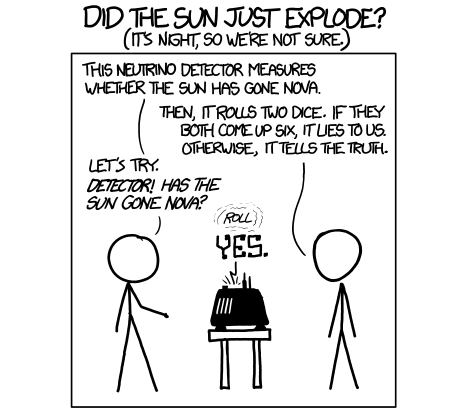
\includegraphics[height=0.8\textheight]{img/frequentists_vs_bayesians-1.png}
  \end{center}

\end{frame}

\begin{frame}
  \frametitle{Ontological Interpretations of Probability}

  \begin{center}
  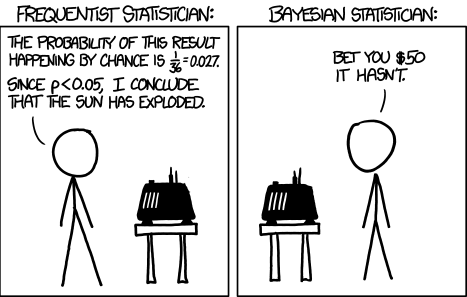
\includegraphics[width=\textwidth]{img/frequentists_vs_bayesians-2.png}    
  \end{center}

\end{frame}

\begin{frame}
  \frametitle{Ontological Interpretations of Probability}
  
  
  \begin{itemize}
  \item Types of Probability
    \begin{itemize}
    \item Frequentist (Classical)
    \item Bayesian (Subjective)
    \end{itemize}
  \item Probability of one-off events
  \item Beliefs of actors
  \item Mathematically equivalent rules
  \end{itemize}

\end{frame}


\begin{frame}
  \frametitle{Probability Distributions}

  \begin{itemize}
  \item Discrete probability: Bernoulli, binomial, geometric, Poisson, 
  \item Continuous probability: normal, Student's t
  \item Parameters
  \item Moments
  \item Support
  \end{itemize}

\end{frame}

\end{document}

%%% Local Variables:
%%% mode: latex
%%% TeX-master: t
%%% End:

%  LocalWords:  DGP dgp SMISS
